\section{Triangles}

Intuition should suggest that there is a fundamental relationship between the lengths of the sides of a triangle, and its interior angles.  There simply aren't enough degrees of freedom in a triangle to allow every side and every angle to be independent, so there must be some relationship between the two.  Using trigonometry, we find that there are indeed two quite useful relationships, known as the law of sines and the law of cosines.\\

\subsection{Properties of triangles}

A quick review of geometric properties of trianges:\\

\begin{enumerate}

\item{A triangle has three sides, and three interior angles.}\\

\item{A the sum of the interior angles of a triangle is $180\degree$, or $\pi\rad$.}\\

\item{The length of any side of a triangle, is less than the sum of the lengths of the other two sides.  For a triangle with sides of lengths $A, B, C$:\\$A < B + C$, $B < A + C$, and $C < A + B$.}\\

\item{A triangle with one interior angle of $90\degree$, or $\frac{\pi}{2}\rad$ is called a {\bf right triangle}.}\\

\item{A triangle with three equal interior angles is called an {\bf equilateral triangle}.}\\

\item{A triangle with two equal interior angles is called an {\bf isocoles triangle}.}\\

\item{A triangle with no equal interior angles is called a {\bf scalene triangle}.}\\

\end{enumerate}

\subsection{Law of sines}

Let us examine a triangle with sides of length $A$, $B$, and $C$, with opposing interior angles $a$, $b$, and $c$.\\

\begin{figure}[htb]
\center
\caption{A triangle.}
\label{fig:A triangle}
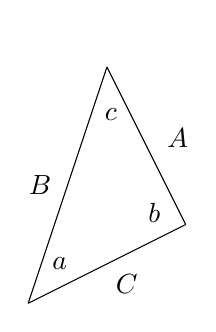
\begin{tikzpicture}[inner sep=0pt,minimum size=0mm]

\node () at (0,3.5) {};

\draw[] (0,0) -- (2,1);
\draw[] (2,1) -- (1,3);
\draw[] (1,3) -- (0,0);

\node () at (0.4,0.5){$a$};
\node () at (1.6,1.15) {$b$};
\node () at (1.05,2.4) {$c$};

\node () at (1.9,2.1){$A$};
\node () at (0.15,1.5) {$B$};
\node () at (1.25,0.25) {$C$};

\end{tikzpicture}
\end{figure}


The {\bf law of sines} states that for a triangle like this, with sides of length $A$, $B$, and $C$, and opposing interior angles $a$, $b$, and $c$, the ratios of the lengths of a side to the sine of the corresponding angle are all equal.  That is:\\

\tab$\frac{sin(a)}{A} = \frac{sin(b)}{B} = \frac{sin(c)}{C}$\\

This holds true for all angles of a triangle, whether acute, right, or obtuse.  A derivation of the Law of Sines can be found in the appendix.\\

\subsection{Law of cosines}

\begin{figure}[htb]
\center
\caption{A triangle.}
\label{fig:A triangle}
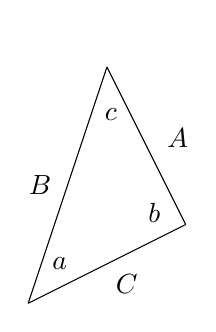
\begin{tikzpicture}[inner sep=0pt,minimum size=0mm]

\node () at (0,3.5) {};

\draw[] (0,0) -- (2,1);
\draw[] (2,1) -- (1,3);
\draw[] (1,3) -- (0,0);

\node () at (0.4,0.5){$a$};
\node () at (1.6,1.15) {$b$};
\node () at (1.05,2.4) {$c$};

\node () at (1.9,2.1){$A$};
\node () at (0.15,1.5) {$B$};
\node () at (1.25,0.25) {$C$};

\end{tikzpicture}
\end{figure}

The {\bf law of cosines} is equally as useful as the law of sines.  The law  of cosines allows you to, given two sides of a triangle and their interior angle, find the length of the third side.  For a triangle of sides $A$, $B$, and $C$, and interior angles of $a$, $b$, and $c$, the law of cosines states that\\

\tab$A^2 = B^2 + C^2 - 2BCcos(a)$\\

This equation should look familiar.  When a is an angle of $\pitwo$ (a right triangle), the cosine term is zero, and the equation reduces to \\

\tab$A^2 = B^2 + C^2$\\

In fact, the law of cosines is a gereralized form of the Pythagorean theorem, for triangles of any angle.  A derivation of the law of cosines can also be found in the appendix.\\

\subsection{Review}

{\begin{figure}[htb]
\center
\caption{A triangle.}
\label{fig:A triangle}
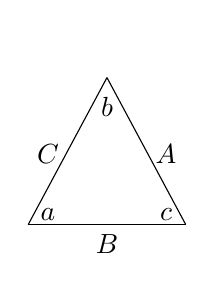
\begin{tikzpicture}[inner sep=0pt,minimum size=0mm]

\node () at (0,2.5) {};

\draw[] (0,0) -- (2,0);
\draw[] (0,0) -- (1,1.866);
\draw[] (2,0) -- (1,1.866);

\node () at (0.25,0.125){$a$};
\node () at (1.0,1.5) {$b$};
\node () at (1.75,0.125) {$c$};

\node () at (1.75,0.9){$A$};
\node () at (0.25,0.9) {$C$};
\node () at (1.0,-0.25) {$B$};

\end{tikzpicture}
\end{figure}
}

\begin{enumerate}

\item{Given $a=b=c=60\degree$ and $A=1$, find $B$ and $C$.}\\

\item{Given $a=35\degree$, $b=55\degree$, and $B=2$, find $c$, $B$, and $C$.}\\

\item{Given $a=45\degree$, $B=2$, and $C=3$, find $A$, $b$, and $c$.}\\

\item{Given $A=5$, $B=7$, $C=13$, find $a$, $b$, and $c$.}\\

\end{enumerate}


